% !TEX root = ../main.tex
% !TEX program = XeLaTeX
% !TEX encoding = UTF-8 Unicode

\date{2018년 3월 7일}

\begin{frontmatter}
\title{마체스어}
\author{최홍범}
\begin{abstract}
Fleck. David W. (2003). A Grammar of Matses, PhD dissertation, Rice University, 1--203.
\end{abstract}
\end{frontmatter}

%%%%%

\section*{발제 범위 분배}
\begin{center}
\begin{tabular}{ccccc}
\hline
1 &최홍범	& Ch. 1--2 	& pp. 1--116 		& 서론, 음운론 \\
2 & 			& Ch. 3--4	& pp. 116--321	& 형태음운론, 형태론 서론, 명사와 대명사 \\
3 &			& Ch. 5		& pp. 322--461	& 동사 \\
4 &			& Ch. 6--7	& pp. 462--624	& 형용사, 부사 \\
5 &			& Ch. 8--9	& pp. 625--750	& 후치사, 조사 \\
6 & 			& Ch. 10--11	& pp. 751--885	& 기본 구 구조, 기본 절 구조 \\
7 &			& Ch. 11		& pp. 885--1000	& 기타 절 구조 \\
8 &			& Ch. 12		& pp. 1001--1188	& 복문 구조 \\
\hline
\end{tabular}
\end{center}

\section{서론}
\subsection{사용 현황}
마체스어는 페루 로레토 주와 브라질 아마조나스 의 아마존 강 상류 지역에서 사용하는 언어로, 화자 수는 2007년 기준 1,720명 내외이다. 사용 인구 수에 비해 언어 사용은 활발하며, EGIDS 척도 상으로는 활발하게 사용되나 가정 및 지역 사회를 넘어선 공식적 사용은 없는 '발전 중' 단계로 분류하고 있다. 
\footnote{Matses | Ethnologue, \textit{Simons, Gary F. and Charles D. Fennig (eds.). 2018. Ethnologue: Languages of the World, Twenty-first edition. }Dallas, Texas: SIL International. Viewed Mar. 6, 2018. https://www.ethnologue.com/language/mcf} 
이 문법서에서는 대부분의 자료를 Gálvez 강 유역의 Nuevo San Juan에서 수집하였다. 

\subsection{`마체스'라는 이름에 대하여}
마체스어를 모국어로 구사하는 사람들은 스스로를 `마체스(영어 Matses, 스페인어/포르투갈어 Matsés)'라 부른다. 단어 `matses'는 발화 맥락에 따라 마체스어 화자만을 지칭하거나 사람 일반을 지칭할 수 있다. Romanoff(1976) 이전의 문헌에서는 `마체스'라는 이름 대신 `마요루나(Mayoruna)'라는 이름을 사용하였다. `마요루나'는 17세기 후반 예수회 사제들이 Huallaga 강과 Javari 강 사이에 사는 사람들을 일컫는 용어였으며 마체스인들은 1969년 SIL과의 접촉 이전에는 해당 명칭을 몰랐다고 한다. 

마체스어에서 `사람'을 지칭하는 단어는 matses `사람, 원주민, 마체스인', mayu `마체스어를 사용하지 않는 원주민', chotac `원주민이 아닌 사람' 세 종류가 있다. 이는 마체스인의 전통적인 선민의식을 드러내지만, 동시에 비마체스인을 인간 이하의 존재로 취급하지도 않았음을 시사한다. 

\begin{table}
\begin{center}
\begin{tabular}{ccc}
\hline
matses	& cun matses		& `우리 사람들(우리 부족)' \\
		& min matses		& `너희 사람들(너희 부족)' \\
		& debin matses	& 'David의 사람들(David의 부족)' \\
mayu	& mayumbo		& `알아들을 수 없는 말을 쓰는 사람들' \\
		& 				& `문명화되지 않은 원주민' 	\\
chotac	& chotac ushu	& `밝은 피부의 비원주민(백인)'	\\

\hline
\end{tabular}
\caption{마체스어의 matses, mayu, chotac 용례}
\end{center}
\end{table}

\subsection{마체스어의 계통}
마체스어는 파노어족(Panoan Languages)에 속한다. Loos(1999)의 파노어족 구분에 따르면 마체스어는 파노어족의 하위집단인 야미나와어파(Yaminawa subgroup), 차코보어파(Chacobo subgroup), 카파나와어파(Capanawa subgroup) 어디에도 속해 있지 않다. Erikson \textit{et al.} (1994)에서는 마체스어를 마티스어(Matis)와 함께 북파노아어파(Northern Panoans) 또는 마요루나 언어들(Mayoruna)
\footnote{Fleck(2003)은 `Mayoruna'의 경우 `Yaminawa subgroup'과 달리 다른 수식을 사용하지 않고 있으므로 마요루나 \textbf{언어들}이라는 표현을 사용하였다.}
로 분류하였다. Erikson \textit{et al.}(1994)과 Fleck(2003)에서 `마요루나'는 마체스어, 마티스어(Matis), 코루보어(Korubo), 쿨리나파노어(Kulina Pano) 등을 포괄하는 개념이다. 마체스어와 마티스어는 53-72\%의 기초어휘를 공유하며, 마체스어 화자에게 마티스어를 들려주었을 때의 이해도는 아주 기초적인 개념을 이해할 수 있을 정도이다. 
\footnote{에스놀로그에서는 마체스어와 마티스어를 묶어 Mayoruna-Matsés로 분류한다. }

\subsubsection{지역 및 사회방언}
\begin{itemize}
\item 마체스어의 방언은 크게 페루 마체스어와 브라질 마체스어로 나눌 수 있다. 이 문법서에서는 페루 마체스어를 다룬다. 
\item 청년층의 언어와 노년층의 언어는 어휘 면에서 큰 차이가 난다. 
\item 노년층은 고어형(archaic)을 발화 시에 사용하기도 한다. 
\item 노년층은 차용보다 마체스식 표현을 사용하는 경향이 있는 반면 청년층은 스페인어 차용어를 사용한다. 
\item 노년층은 차용어를 마체스 음운 구조에 맞추는 반면 청년층은 스페인어 발음을 모방하려 한다. 
\end{itemize}

\subsubsection{다른 언어와의 접촉}
마체스인들은 대부분 마체스어를 모어로 사용하며, 마체스인들이 사로잡은 포로의 자녀들 역시 부모의 모국어가 아닌 마체스어를 주로 사용한다. 페루 마체스인의 경우 대부분 스페인어를 몇 단어 정도 알고 있지만 정확한 스페인어를 구사하지 못한다. 

\subsection{마체스인의 생활}
\subsubsection{자연환경}
마체스인은 대부분 마을에 모여 거주한다. 마을은 대부분 Javari 강과 Gálvez 강가에 위치한다. 기후는 연중 따뜻하며 우기(9월-4월)와 非우기(5월-9월)로 나뉜다. 주변 환경은 열대우림이며 우기에 범람하는 지역과 범람하지 않는 지역으로 나뉜다. 최근에 들어서는 수운이나 수산물 등 강을 적극적으로 이용하지만, 마체스인은 전통적으로는 범람 범위 바깥에서 생활해왔다. 

\subsubsection{식생활}
마체스인은 수렵, 농사, 어로, 목축, 채집 등을 통해 식재료를 조달한다. 
\begin{itemize}
\item 주된 단백질원은 사냥을 통해 얻으며, 페커리(돼지를 닮은 포유류), 맥, 사슴, 원숭이 따위의 동물을 주로 사냥한다. 
\item 농사는 화전을 이용한다. 화전을 통해 뿌리식물과 과일을 길러 탄수화물원으로 삼는다. 
\item 1970년대부터 닭, 돼지, 오리 등을 기르기 시작하였다. 
\item 잉여 식량을 팔아 번 돈으로 의류, 총알, 낚시도구 등을 구매한다. 
\end{itemize}

\subsubsection{그 외 특징}
\begin{itemize}
\item 사촌 간 결혼 및 일부다처제가 가능하다. 
\item 남녀 분업이 뚜렷한 반면 직업의 분업은 이루어지지 않았다. 
\item 죽은 자의 이름과 비슷한 단어를 금기시(피휘)하는 풍습이 있다. 그러나 신화에 등장하는 단어에는 적용되지 않는다. 
\item 마을 간 교류가 존재하나, 페루 마체스 마을과 브라질 마체스 마을 사이에는 교류가 거의 없다. 
\end{itemize}

\section{음운론}
\subsection{음소 목록}
마체스어는 자음 음소 15개, 모음 음소 6개 총 21개의 음소를 가지고 있다. 
\subsubsection{자음}
마체스어의 자음은 아래와 같다. 괄호 안의 표기는 전사를 위한 표기이다:  

\begin{center}
\begin{tabular}{|c|c|c|c|c|c|c|}
\hline
			& labial	& alveolar	& retroflex	& palatal	& velar	\\ \hline
stop			& p b	& t d 		& 			&		& k (c/qu)	\\ \hline
nasal		& m		& n			&			&		& 		\\ \hline
fricative		& 		& s			& ʂ (sh)		& ʃ (sh)	&		\\ \hline
affricate		& 		& ts			& tʂ (ch)		& tʃ (ch)	&		\\ \hline
approximant	& w (u)	&			&			& j (y)	&	 	\\
\hline
\end{tabular}
\end{center}

\subsubsection{자음의 조건부 음 변화 및 환경 제약}
\begin{itemize}
\item 파열음
	\begin{itemize}
	\item /d/는 모음 사이에서 [ɾ]로 실현되며
		\footnote{Fleck(2003)은 이 변이음을 권설 탄음으로 기술하고 있다. 권설 탄음의 IPA 표기는 [ɽ]이지만 발제문에서는 원문의 표기를 사용한다.}
		어말에서는 불파음 [d̚]으로 실현된다. 
	\item /k/는 음절 말에서 성문 파열음 [ʔ]으로 실현된다.
	\item 비모음 /n/은 뒤따르는 파열음과의 역행자음동화를 통해 [m] 또는 [ŋ]으로 실현된다. 그러나 /nm/은 [nm]으로 실현된다. 
	\item 중복 자음은 어절 가운데, 형태소 내부 또는 경계에 나타날 수 있으며, /kk/ [ʔk]와 /nn/ [nn]에 한한다. 
	\end{itemize}
\item 마찰음
	\begin{itemize}
	\item 중복 자음은 /ss/, /ʂʂ/, /ʃʃ/ 모두 어절 가운데, 형태소 경계에 나타난다. /kk/, /nn/과 달리 형태소 내부에는 나타나지 않는다. 
	\end{itemize}
\item 파찰음
	\begin{itemize}
	\item 무성 권설 파찰음 /tʂ/는 후설 모음 및 중설 고모음 앞에서만 나타난다. 무성 구개 파찰음 /tʃ/는 모든 환경에서 나타나며 최소대립쌍이 존재하므로 /tʂ/와 /tʃ/는 독립된 음소로 분류한다. 
	\end{itemize}
\item 접근음
	\begin{itemize}
	\item 이 문법서에서는 \textbf{접근음} /j/, /w/와 \textit{반모음} [j](/i/), [w](/u/)를 구분하여 기술하고 있다. 이에 대해서는 후술한다. 
	\item /w/에는 원순성이 없음에 유의하라. 
	\end{itemize}
\end{itemize}

\subsubsection{모음}
마체스어의 모음은 아래와 같다. 괄호 안의 표기는 전사를 위한 표기이다:  

\begin{center}
\begin{tabular}{|c|c|c|c|}
\hline
	& front	& central	& back	\\ \hline
high	& i 		& ɨ  (ë)	& ɯ	(u)	\\ \hline
mid	& e		& 		& ɤ	(o)	\\ \hline
low	& 		& a 		&		\\
\hline
\end{tabular}
\end{center}

\begin{itemize}
\item 모음의 비음성, 장단은 변별적이지 않다. 
\item 단어 단위의 강세는 변별적이나 발화 단위의 강세는 변별적이지 않으며 발화의 마지막 음절에 위치한다. 
\end{itemize}

\subsubsection{모음의 조건부 음 변화 및 환경 제약}
\begin{enumerate}
\item /e/는 자유변이음 [ɛ]와 연속체를 이룬다. 개음절의 경우 발음이 [e]에 가까우며 성문 파열음 [ʔ] 앞에 올 때는 [ɛ]에 가깝게 발음된다. 

\begin{figure}
	\centering
		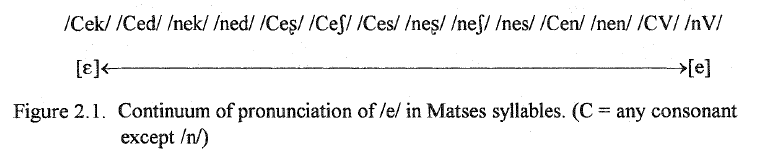
\includegraphics[width=100mm]{Matses/src/matses1.png}
		\caption{여러 환경에서 마체스어 /e/의 발음 스펙트럼}
\end{figure}
\item 모든 모음은 비자음 앞에서 비음화된다. 
\item /i/, /u/는 모음 앞뒤에서 반모음 [j], [w]로 실현된다. /i/와 /u/가 인접할 경우 상승 이중모음으로 실현된다. 즉, /ui/는 [wi], /iu/는 [ju]로 실현된다.  
\item 형태소 경계에서 /e/, /o/는 반모음 [j], [w]으로 상승하기도 한다. 이에 대해서는 후술한다. 
\end{enumerate}

\subsection{음절 구조}
마체스어의 음절 구조는 최대 CVVVC의 구조를 가진다. 이는 반모음의 기저형을 자음으로 둘지 모음으로 둘지에 따라 달라지며, 각각의 경우에 따른 음절 구조 분석은 아래 도표와 같다: 
\footnote{Fleck(2003)에서는 반모음 [j], [w]의 기저형을 모음 /i/, /u/로 설정하고 Dorigo(2001)에서는 기저형을 자음 [j], [w]로 설정하여 음절구조 분석을 진행하였다.}

\begin{figure}
	\centering
		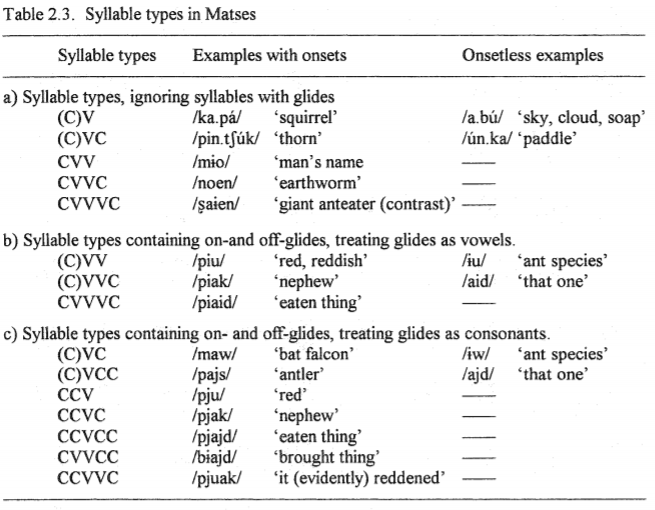
\includegraphics[width=100mm]{Matses/src/matses2.png}
		\caption{반모음 [j], [w]의 기저형 설정에 따른 마체스어의 음절 구조 분석}
\end{figure}

\begin{itemize}
\item 마체스어의 어절은 위에 나타나는 음절을 임의로 조합한 형태로 나타난다. 단, 초성이 없는 V, VC, VV, VVC와 같은 음절 구조는 어절 앞에만 나타날 수 있다. 
\item 논리적으로 가능한 이중모음의 조합 36개 중 실제로 나타나는 이중모음은 24개이다. 그 중 7개는 형태소 경계에서 음운 변화를 통해서만 나타난다. 마체스어의 이중모음은 아래 도표에 나타난 바와 같다:
\footnote{아래첨자\textsubscript{m}은 해당 이중모음이 형태론 경계에서만 관찰이 가능함을 의미하며, \*는 형태음운 변화에 의해 다른 (이중)모음으로 실현됨을 의미한다. ?는 해당 이중모음이 관찰된 바 없음을 나타낸다.}

\begin{figure}
	\centering
		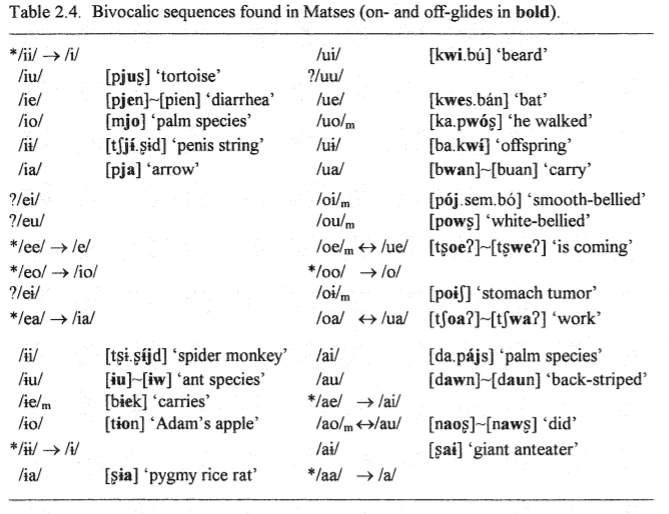
\includegraphics[width=100mm]{Matses/src/matses3.png}
		\caption{마체스어의 이중모음}
\end{figure}
\end{itemize}

마체스어는 어두 자음군을 허용하지 않지만 자음군은 제한적으로 허용한다. 마체스어에 나타나는 자음군은 아래 도표와 같다. \textbf{굵은} 글자는 해당 자음군이 형태소 경계에서만 나타남을 의미한다: 

\begin{figure}
	\centering
		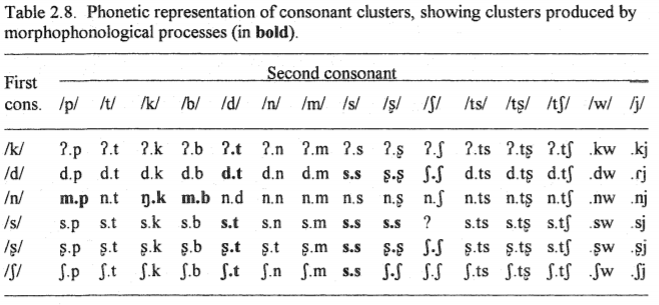
\includegraphics[width=100mm]{Matses/src/matses4.png}
		\caption{마체스어의 자음군}
\end{figure}